\documentclass[11pt,a4paper]{ctexart}
\usepackage{fontspec}
\defaultfontfeatures{Mapping=tex-text}
\usepackage{xunicode}
\usepackage{xltxtra}
%\setmainfont{???}
\usepackage{amsmath}
\usepackage{amsfonts}
\usepackage{amssymb}
\usepackage{graphicx}
\usepackage{amsthm}
\usepackage{array}
\usepackage{float}   %{H}
\usepackage{booktabs}  %\toprule[1.5pt]
\usepackage[titletoc]{appendix}
\usepackage{tcolorbox} %彩色框框
%===================%插入代码需要的控制
\usepackage{listings}
\usepackage{listings}
\usepackage{xcolor}
\setmonofont{Consolas}%字体
\lstset{
	numbers=left, 
	numberstyle= \tiny, 
	keywordstyle= \color{ blue!70},
	commentstyle= \color{red!50!green!50!blue!50}, 
	frame=shadowbox, % 阴影效果
	rulesepcolor= \color{ red!20!green!20!blue!20} ,
	escapeinside=``,% 英文分号中可写入中文
	basicstyle=\ttfamily 
} 
%===================%
\usepackage[left=2cm,right=2cm,top=2cm,bottom=2cm]{geometry}

\newtheorem{theorem}{定理}
\newtheorem{definition}{定义}
\newtheorem*{solution}{解}

\title{定性数据统计分析作业 (2)}
\author{钟瑜 \quad 222018314210044}
\date{\today}
\begin{document}
\maketitle
\pagestyle{plain}%设置页码
%==================================================================================%
\begin{figure}[H]
	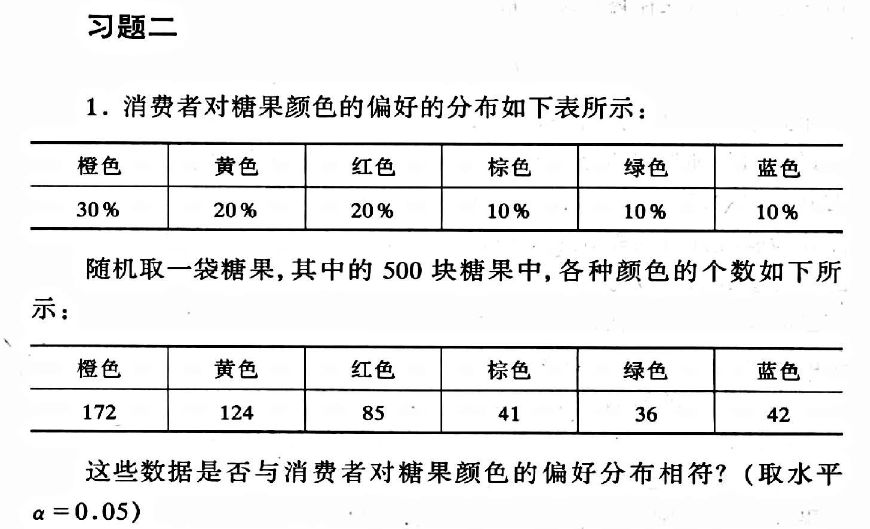
\includegraphics[width=0.7\textwidth]{1.png}
\end{figure}

\begin{solution}
R代码如下:
\end{solution}
\begin{lstlisting}[language=r]
> x<-c(172,124,85,41,36,42)
> p<-c(0.3,0.2,0.2,0.1,0.1,0.1)
> n<-sum(x)
> chi<-sum((x-n*p)*(x-n*p)/(n*p)) 

> p_value=1-pchisq(chi,5);
> p_value   
[1] 0.002876218

#或者
> chisq.test(x,y=NULL,correct =TRUE,p=p)

Chi-squared test for given probabilities

data:  x
X-squared = 18.057, df = 5, p-value = 0.002876
\end{lstlisting}
p值小于$ \alpha $=0.05,故这些数据确实与消费者对糖果颜色的偏好不相符.


\begin{figure}[H]
	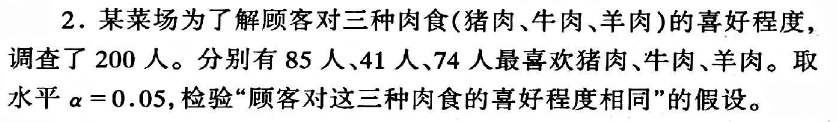
\includegraphics[width=0.7\textwidth]{2.png}
\end{figure}
\begin{solution}
R代码如下:
\end{solution}
\begin{lstlisting}[language=r]
> x<-c(85,41,74)
> chisq.test(x,y=NULL,correct = TRUE,p=rep(1/length(x),length(x)))

Chi-squared test for given probabilities

data:  x
X-squared = 15.73, df = 2, p-value = 0.0003839
\end{lstlisting}
p值小于$ \alpha $=0.05, 故顾客对这三种肉食的喜好程度不相同.

%=================================================================================%
\newpage
\centering\textbf{\Large 附录}
\begin{appendices}


\section{关于卡方分布的函数说明}
\begin{tcolorbox}[colback=blue!7!white,colframe=blue!40]
\textbf{The (non-central) Chi-Squared Distribution}

\textbf{Description}\\
Density, distribution function, quantile function and random generation for the chi-squared ($chi^2$) distribution with df degrees of freedom and optional non-centrality parameter ncp.

\textbf{Usage}\\
dchisq(x, df, ncp = 0, log = FALSE)\\
pchisq(q, df, ncp = 0, lower.tail = TRUE, log.p = FALSE) 卡方随机变量的累积分布函数\\
qchisq(p, df, ncp = 0, lower.tail = TRUE, log.p = FALSE)\\
rchisq(n, df, ncp = 0)\\


dchisq gives the density, \\
pchisq gives the distribution function, \\
qchisq gives the quantile function, \\
rchisq generates random deviates.

\textbf{Arguments}\\
x, q:	vector of quantiles.

p:	vector of probabilities.

n:	number of observations. If length(n) > 1, the length is taken to be the number required.

df:	degrees of freedom (non-negative, but can be non-integer).

ncp:	non-centrality parameter (non-negative).

log, log.p:	logical; if TRUE, probabilities p are given as log(p).

lower.tail:	logical; if TRUE (default), probabilities are P[X$ \leq $x], otherwise, P[X > x].
\end{tcolorbox}

\section{关于卡方检验的函数说明}
\begin{tcolorbox}[colback=blue!7!white,colframe=blue!40]
\textbf{Pearson's Chi-squared Test for Count Data}

\textbf{Description}\\
chisq.test performs chi-squared contingency table tests and goodness-of-fit tests.

\textbf{Usage}\\
chisq.test(x, y = NULL, correct = TRUE,
p = rep(1/length(x), length(x)), rescale.p = FALSE,
simulate.p.value = FALSE, B = 2000)

\textbf{Arguments}\\
x:	a numeric vector or matrix. x and y can also both be factors.

y:	a numeric vector; ignored if x is a matrix. If x is a factor, y should be a factor of the same length.

correct:	a logical indicating whether to apply continuity correction when computing the test statistic for 2 by 2 tables: one half is subtracted from all |O - E| differences; however, the correction will not be bigger than the differences themselves. No correction is done if simulate.p.value = TRUE.

p:	a vector of probabilities of the same length of x. An error is given if any entry of p is negative.

rescale.p:	a logical scalar; if TRUE then p is rescaled (if necessary) to sum to 1. If rescale.p is FALSE, and p does not sum to 1, an error is given.

simulate.p.value:	a logical indicating whether to compute p-values by Monte Carlo simulation.

B:	an integer specifying the number of replicates used in the Monte Carlo test.
\end{tcolorbox}

\end{appendices}


\end{document}